\chapter{Переход Фредерикса при отрицательной анизотропии диэлектрической проницаемости.}\label{ch:ch4}

Ячейки ЖК с отрицательной анизотропией диэлектрической проницаемости отличаются тем, что, находясь во внешнем электрическом поле, молекулы ЖК стремятся выстроиться не вдоль его силовых линий, а поперёк.
Это связано со знаком $\varepsilon_a$: при $\varepsilon_a < 0$ энергия электрического поля в диэлектрике, даваемая формулой~\eqref{E_field}, становится минимальной, когда $\theta(z) = \pi/2$ на интервале $z\in [0,L]$.
Для анализа равновесной ориентационной структуры в ячейке ХЖК с отрицательной анизотропией диэлектрической проницаемости ($\varepsilon_a < 0$) вновь обратимся к методу численной минимизации функционала свободной энергии $\FF_\mathrm{tot}$.
Процедура минимизации функционала свободной энергии $\FF_\mathrm{tot}$ аналогична таковой, использованной в работе~\cite{OskirkoPRE2018}, и организована следующим образом: 

аналогично таковой в главе~\ref{ch:ch2}: представим угол $\theta(z)$ в виде
\begin{equation}\label{eq:psi+Fourier}
\theta(z) = \pi/2 +
\delta_1\frac{\sinh \xi(L-z)}{\sinh\xi L}+\delta_2\frac{\sinh\xi z}{\sinh\xi L}
+ \sum\limits_{n=1}^N c_n\sin(\pi nz/L),
\end{equation}





где  $\xi = \sqrt{\left(K_{33}q_0^2-\varepsilon_a U^2/(4\pi L^2)\right)K_{11}^{-1}}$ имеет размерность обратной длины, коэффициенты $\delta_1$, $\delta_2$  и $c_n$,  $n=1,\dots,N$ являются изменяемыми параметрами.
При этом уравнение~\eqref{eq:gran-1} позволяет сократить на 2 количество независимых параметров, а уравнение~\eqref{eq:theta'} используется для контроля точности работы минимизационного алгоритма.


\todo{Начало вставки}

Равновесную ориентационную структуру в ячейке ХЖК будем искать с помощью численной минимизации свободной энергии~\eqref{eq:F_for_minimization}, используя следующие углы лёгкого ориентирования на границах:
\begin{equation}\label{eq:initial}
\theta_0^{(1)}=\theta_0^{(2)}={\pi}/{2},\;\phi_\mathrm{tot}^{(0)}=q_0L.
\end{equation}
Эти условия соответствуют ненапряжённому ХЖК в отсутствие внешнего электрического поля.
Сведём задачу поиска минимума функционала $\FF_\mathrm{tot}[\theta(z)]$ к задаче поиска минимума функции нескольких переменных, аппроксимировав искомую зависимость $\theta(z)$ пробной функцией
\begin{equation}\label{eq:psi+Fourier}
\theta(z) =
\pi/2 + {\delta\psi}(z,\delta_1,\delta_2) + \sum\limits_{n=1}^N c_n\sin(\pi nz/L).
\end{equation}
Здесь слагаемое $\pi/2$ соответствует неискажённому состоянию.
Функция $\delta\psi(z,\delta_1,\delta_2)$, задаваемая выражением~\eqref{psi=}, содержит $\delta_1$ и $\delta_2$ -- отклонения от углов лёгкого ориентирования на границах: $\theta(0) = \pi/2 + \delta_1$, $\theta(L) = \pi/2 + \delta_2$.
Наконец, ряд Фурье описывает объёмные искажения ориентационной структуры, не затрагивающие границы.
Используя граничные условия~\eqref{eq:gran-1}, можно выразить коэффициенты $c_N$ и $c_{N-1}$ через все остальные -- $\delta_{1,2}$ и $\{c_n\}_{n=1}^{N-2}$.
Таким образом, углы $\delta_1$, $\delta_2$, а также коэффициенты $c_n$, $n=1,\dots,N-2$ являются регулируемыми параметрами.

Ограничимся в~\eqref{eq:psi+Fourier} $N = 20$ членами ряда Фурье.
Учёт более, чем 20 слагаемых приводит к относительному изменению профиля $\theta$ менее чем на $0.5\%$ для любого $z$ на всём интервале $[0,\, L]$.
В многомерной численной минимизации существует проблема попадания в максимумы или в седловые точки.
Для того, чтобы определить, действительно ли минимизация свободной энергии привела к минимуму, используем случайные небольшие сдвиги параметров  $\delta_{1,2}$, $\{c_n\}$ относительно полученных значений.
Если минимизационный алгоритм приводит к другому ответу, это означает, что предыдущий результат был ошибочным -- максимумом или седловой точкой.
При этом в случае, если достигнут, по крайней мере, локальный минимум, то при любом достаточно небольшом сдвиге минимизация будет всегда возвращать нас обратно.

Будем изменять напряжение $U$, зафиксировав все остальные параметры ячейки ЖК.
\begin{figure}
	\centering
	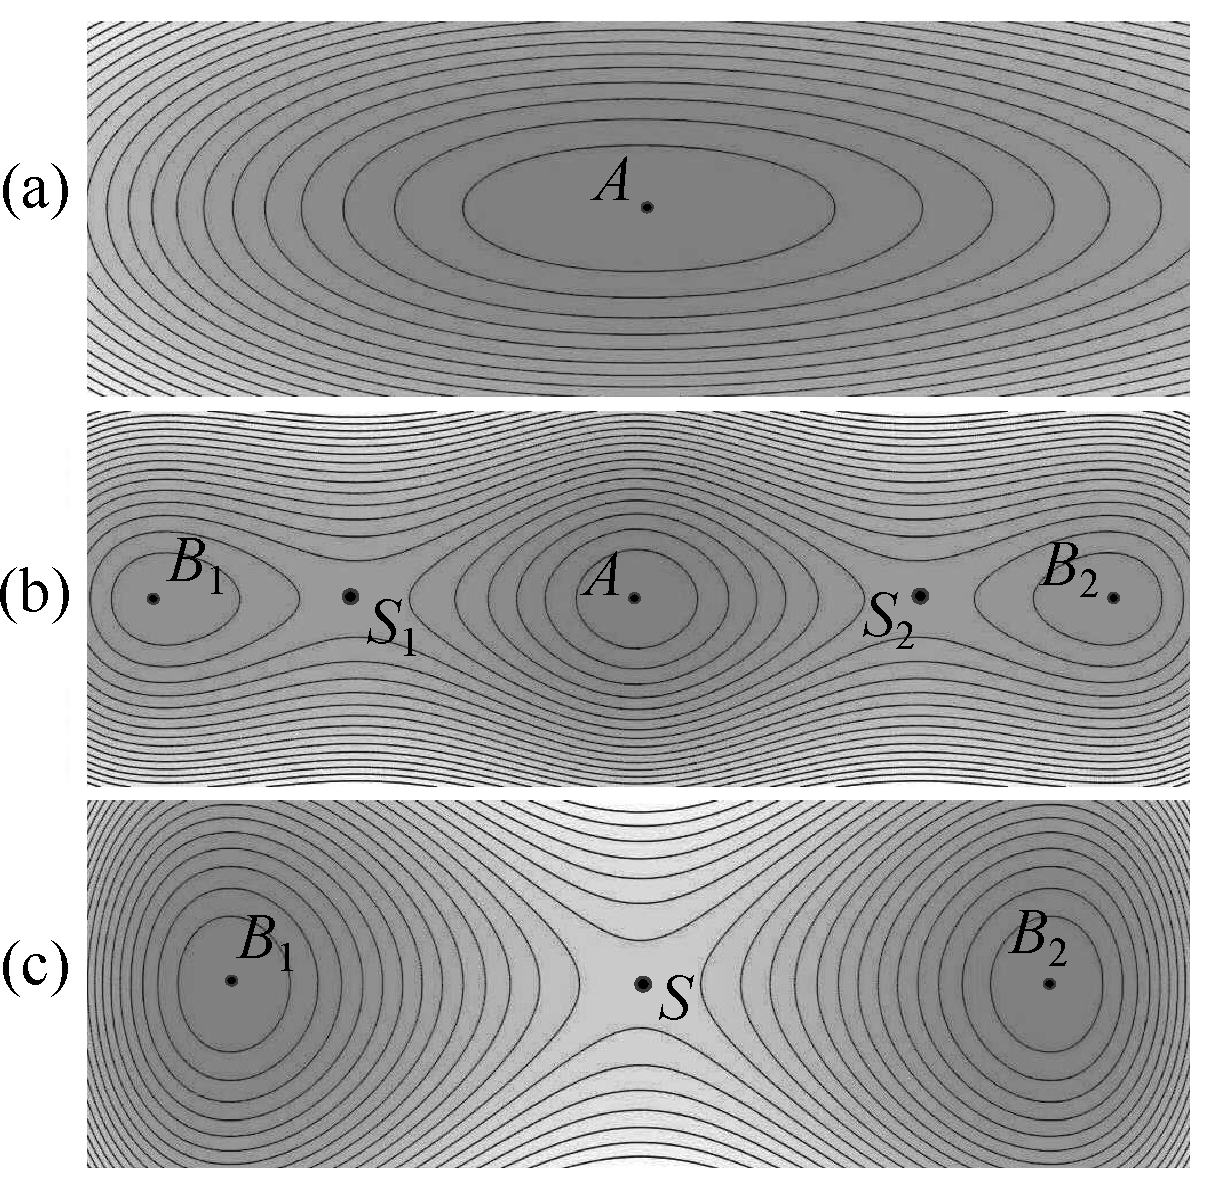
\includegraphics[width = 15cm]{Geo_final.eps}
	\caption{Схематичное двумерное изображение случаев, возникающих при численной минимизации свободной энергии}
	\label{pic_Geo_final}
\end{figure}
При этом будет наблюдаться один из трёх случаев, проиллюстрированных на Рис.~\ref{pic_Geo_final}:
\begin{enumerate}
	\item[(a)]
	Существует единственный минимум (точка А на рис.~\ref{pic_Geo_final}a), соответствующий планарной геликоидальной структуре, при этом $\delta_{1,2}=0$, $c_n = 0$, то есть $\theta(z)=\pi/2$, а $\phi(z) = q_0z$.
	\item[(b)]
	Случай трёх минимумов.
	Один из них (точка А на Рис.~\ref{pic_Geo_final}b) по-прежнему соответствует планарной геликоидальной структуре.
	Два других (точки $B_1$ и $B_2$) соответствуют искажённым структурам, то есть таким, для которых некоторые из параметров $\delta_{1,2}$, $c_n$ ненулевые.
	При этом параметры $(\delta_{1},\delta_{2},c_n)$, соответствующие точкам $B_1$ и $B_2$, отличаюся только знаком, следовательно, этим двум точкам соответствуют одинаковые распределения директора ввиду симметрии относительно замены ${\bf n} \leftrightarrow -{\bf n}$.
	\item[(c)]
	Имеются ровно два минимума.
	В этом случае существуют два минимума $B_1$ и $B_2$, соответствующие одной и той же искажённой ориентационной структуре.
	Планарная геликоидальная структура здесь не существует, так как является седловой точкой ($S$ на Рис.~\ref{pic_Geo_final}c).
\end{enumerate}
Здесь и далее мы будем называть ''устойчивыми'' равновесные состояния, соответствующие локальным минимумам свободной энергии, а ''метастабильными'' -- устойчивые состояния с энергией, большей, чем у другого устойчивого состояния.

\subsubsection{"Фазовая" \todo{(Структурная?)} диаграмма}

Случай (a) на Рис.~\ref{pic_Geo_final} возникает для напряжений $|U|$ ниже порогового значения $U^{**}$, а при достижении этого значения могут наблюдаться две различные ситуации.
Они соответствуют разрывному (I) и непрерывному (II) переходу Фредерикса:
\begin{itemize}
	\item[I.]
	В этом случае существует ещё одно пороговое значение $U^{*} > U^{**}$, при этом для $|U|\in (U^{**},\, U^{*})$ у функционала свободной энергииесть сразу три локальных минимума, из которых один соответствует начальной планарной геликоидальной структуре	, а два других -- искажённой ориентационной структуре, как показано на Рис.\ref{pic_Geo_final}b.
	Здесь $U^{**}$ -- наименьшее напряжение, при котором искажённая ориентационная структура ещё может существовать в качестве метастабильной, а, в свою очередь, $U^{*}$ -- максимальное напряжение, при котором планарная геликоидальная структура ещё может существовать как метастабильная.
	Таким образом, при любом $U$ из интервала $(U^{**},\,U^*)$ только одна из структур будет стабильной (с меньшей энергией), в то время как другая будет метастабильной.
	С ростом напряжения $|U|$ свободная энергия искажённой структуры уменьшается, и при $|U| = U_c$ становится равной энергии неискажённого состояния, и происходит разрывный переход Фредерикса.
	То есть, при $|U| < U_c$ более энергетически выгодным является неискажённое состояние, а при $|U| > U_c$ -- искажённое.
	Наконец, при $|U|>U^*$ реализуется случай (c).
	\item[II.]
	В данном сценарии существует только одно пороговое напряжение, $|U| = U_c$. Этот сценарий соответствует (I) для $U^{*} = U_c = U^{**}$, при этом происходит непрерывный переход Фредерикса. 
	Здесь при $|U| < U_c$ возникает случай (a), а при  $|U|>U_c$ -- случай (c), показанные на Рис.~\ref{pic_Geo_final}c.
\end{itemize}
Интервалы стабильности и метастабильности схематично изображены на Рис.~\ref{pic-U*U**Uc_otline}.
\begin{figure}%[thb]
	\centering
	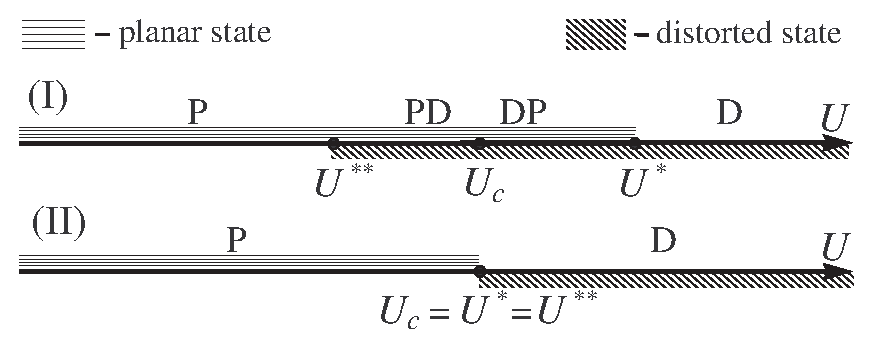
\includegraphics[width=12cm]{UU1d3a.eps}
	\caption{Иллюстрация разрывного (I) и непрерывного (II) переходов Фредерикса для $U > 0$.
		(I): Области устойчивости искажённой (D) структуры, $U>U^{**}$, и неискажённой (P) структуры, $U<U^{*}$.
		На интервале, обозначенном PD, $U^{**}<U<U_c$, искажённая структура метастабильна, а на интервале DP, $U_c < U < U^{*}$, метастабильна планарная геликоидальная структура.
		(II):  Области устойчивости для искажённой, $U > U_c$, и неискажённой структуры, $U < U_c$.}
	\label{pic-U*U**Uc_otline}
\end{figure}

Для того, чтобы изучить, как влияет флексоэлектрическая поляризация на переход Фредерикса, были рассчитаны пороговые напряжения $U^{**}$, $U_c$, $U^{*}$ для различных значений усреднённого флексоэлектрического коэффициента $\bar{e}$.
Отметим, что учёт флексоэлектричества привёл к тому, что значения напряжений $U^{**}$, $U^*$ и $U_c$ стали различными для  $U>0$ и $U<0$, если константы сцепления с подложкой различны, $W_\theta^{(1)}\not=W_\theta^{(2)}$.
Значения материальных констант были взяты такими же, как и в~~\cite{VAR2013}: $K_{11}=0.42\times 10^{-6}$~дин, $K_{22}=0.23\times 10^{-6}$~дин, $K_{33}=0.53\times 10^{-6}$~дин,  $q_0=500$~$\text{cm}^{-1}$, $L=60$~$\mu\text{m}$, $W_\theta^{(1)}=2.5\times 10^{-3}$~эрг/см$^2$, $W_\theta^{(2)}=0.5\times 10^{-3}$~эрг/см$^2$,  $W_\phi^{(1)}=2.5\times 10^{-4}$~эрг/см$^2$, $W_\phi^{(2)}=1.0\times 10^{-4}$~эрг/см$^2$, $\varepsilon_\bot=7.2$, $\varepsilon_\|=16.2$.
\todo{В дальнейшем будем называть этот набор параметров стандартным.}
Выбранные значения параметров $q_0$ и $L$ соответствуют супертвист-ячейке ЖК с полной закруткой $q_0L = 3>\pi/2$.
Кроме того, значения констант сцепления с подложкой выбраны сильно различающимися, чтобы продемонстрировать влияние такой асимметрии границ.
На Рис.~\ref{pic-U_from_e_pos} представлена рассчитанная "фазовая диаграмма" в координатах ($\bar{e}$, $U$) для обоих направлений электрического поля.
\begin{figure}%[bht]
	\centering
	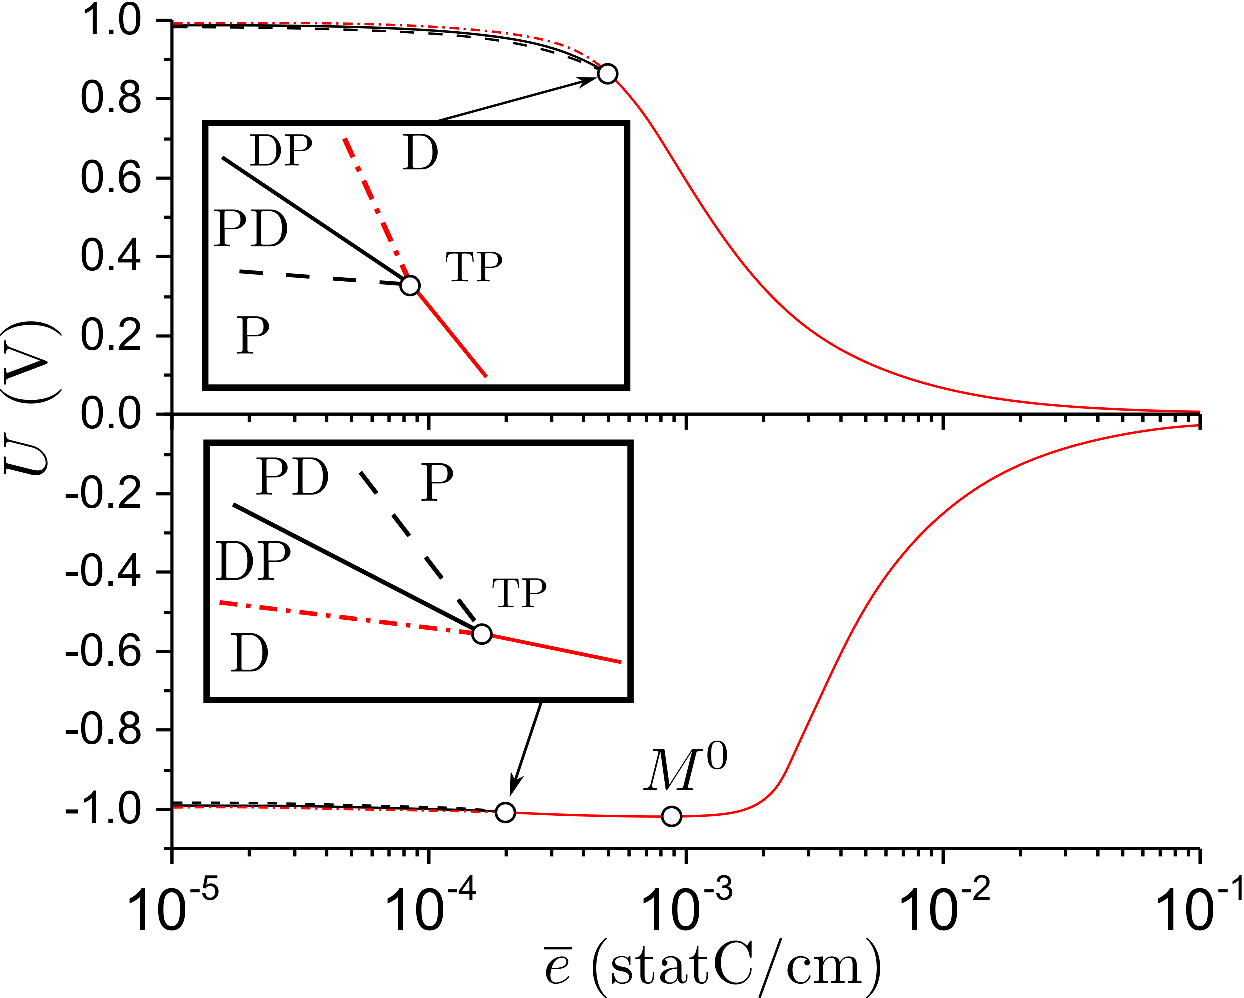
\includegraphics[width=15cm]{Graph7colorB.eps}
	\caption{Фазовая диаграмма.
		Напряжения $U^*$, $U_c$ и $U^{**}$ как функции усреднённого флексоэлектрического коэффициента $\bar{e}$: пунктирная линия -- $U^{**}$, сплошная линия -- $U_c$, штрихпунктирная линия -- $U^{*}$.
		Области стабильности и метастабильности обозначены на вставках.
		Трикритические точки обозначены как TP, другие обозначения совпадают с таковыми на Рис.~\ref{pic-U*U**Uc_otline}.
		Правее трикритической точки TP линии $U^*$, $U_c$ и $U^{**}$ совпадают.}
	\label{pic-U_from_e_pos}
\end{figure}






\todo{Конец вставки}

При помощи минимизации свободной энергии были найдены равновесные ориентационные структуры в ячейке ХЖК при различных значениях усреднённого флексоэлектрического коэффициента $\bar{e}$ и приложенного напряжения $U$, а также следующих значениях материальных констант: $K_{11}=0.42\times 10^{-6}$~дин, $K_{22}=0.23\times 10^{-6}$~дин, $K_{33}=0.53\times 10^{-6}$~дин,  $q_0=500$~$\text{cm}^{-1}$, $L=60$~$\mu\text{m}$, $W_\theta^{(1)}=2.5\times 10^{-3}$~эрг/см$^2$, $W_\theta^{(2)}=0.5\times 10^{-3}$~эрг/см$^2$,  $W_\phi^{(1)}=2.5\times 10^{-4}$~эрг/см$^2$, $W_\phi^{(2)}=1.0\times 10^{-4}$~эрг/см$^2$, $\varepsilon_\bot=16.2$, $\varepsilon_\|=7.2$.
Заметим, что от стандартного набора параметров этот набор отличается только значениями диэлектрической проницаемости $\varepsilon_\bot$ и $\varepsilon_\|$.

Полученные результаты для $\varepsilon_a < 0$ для сравнения приводятся вместе с аналогичными результатами для $\varepsilon_a > 0$. На Рис.~\ref{fig1} на плоскости $(\bar{e},U)$ приведены рассчитанные области устойчивости планарной геликоидальной ориентационной структуры.
\begin{figure}
	\centering
	\includegraphics[width=0.49\textwidth]{1aa.eps}%{PhD_negative_ea.png}\hspace{2pc}%
	\hfill
	\includegraphics[width=0.49\textwidth]{1bb.eps}%{PhD_negative_ea.png}\hspace{2pc}%
	\caption{Фазовые диаграммы для случаев $\varepsilon_a < 0$ и $\varepsilon_a > 0$. Сплошной и пунктирной линией обозначена граница между различными "фазами" при разрывном и непрерывном переходе соответственно.
		Точечной линией обозначена асимптота межфазовой границы при $\varepsilon_a < 0$, а знаком ``$\circ$'' -- трикритическая точка.}\label{fig1}
\end{figure}
Данный результат можно получить и аналитически аналогично тому, как это было проделано в Главе~\ref{ch:ch3}.
Для этого следует изучить знак второй вариации функционала свободной энергии на планарной геликоидальной структуре $\delta^2 \FF_\mathrm{tot}(\theta_0,\phi_0)$.
При этом вклад, связанный с вариацией $\phi$, всегда неотрицателен, а вклад, связанный с вариацией $\theta$, даётся формулой~\eqref{d2F_theta}.
Важным отличием от случая $\varepsilon_a > 0$ является то, что $M > 0$ при любых значениях напряжения $U$.
Это приводит к тому, что после выполнения разбиения $\delta^2\FF_\theta = (Q_\mu + Q_\psi)S_\bot/2$ первое слагаемое оказывается всегда неотрицательным.
Приведём явный вид $Q_\psi$ для случая $\varepsilon_a < 0$:
\begin{equation}
Q_\psi = \sum\limits_{\alpha=1,2}\left(K_{11}\xi \coth{\xi L}+\EuScript{W}^{(\alpha)}\right) \delta_\alpha^2\\
- 2K_{11} (\xi/\sinh\xi L)\delta_1\delta_2,
\end{equation}
$\xi$ задаётся формулой~\eqref{xi=}.
Требование положительности $Q_\psi$ приводит к третьему неравенству в~\eqref{eq:ineq_M>0_final_c}:
\begin{equation}
w^{(1)} w^{(2)} + 2\bar{w} t \coth{t} + t^2 > 0,
\end{equation}
где $t = \xi L$.
Это нервенство квадратично относительно $\bar{e}$, и его решение даётся неравенствами~\eqref{eq:interval_1} и~\eqref{eq:interval_2} при $U_1\to\infty$.
Приведём явный вид решения:
\begin{align}
&0\leq \bar{e}\leq+\infty,\!  &&\text{если }U = 0,\\
&0\leq \bar{e} < e_+^*,\!  &&\text{если }0<|U|<\infty,
\end{align}
где
\begin{equation}\label{eq:e(U)_ea<0}
e_+^*(U)=\left(K_{11}/4U\right)\left(\Delta{w}
+ 2\bar{w}\sgn{U}\sqrt{ 1+X(U) }\right) ,
\end{equation}
\begin{equation}\label{eq:X(U)_ea<0}
X(U)=\frac{2}{\bar{w}}\left( t\coth t +{t^2}/2\bar{w}\right).
\end{equation}
Кривая $e^*_+(U)$, построенная по выражению~\eqref{eq:e(U)_ea<0}, совпадает с расчётной кривой $U^*(\bar{e})$.
Кроме того, можно рассчитать положение вертикальной асимптоты $\bar{e}'$:
\begin{equation}
\bar{e}' = \lim_{U\to \infty} \bar{e}^*_+(U) = \sqrt{\frac{-\ve_a K_{11}}{16\pi}}
\end{equation}
Подставляя указанные выше значения параметров, получаем $\bar{e}' =2.74\times 10^{-4} $~Фр/см, что также хорошо согласуется с численными расчётами.

Отметим важные свойства диаграммы в случае $\varepsilon_a < 0$.
С одной стороны, переход Фредерикса оказывается невозможен при небольших значениях $\bar{e}$.
Этот результат, в частности, согласуется с эмпирическим представлением о том, как должны выстраиваться молекулы с отрицательной анизотропией диэлектрической проницаемости во внешнем электрическом поле в отсутствие флексоэлектрической поляризации.
С другой стороны, существует некоторое значение $\bar{e}'$ такое, что при $\bar{e} > \bar{e}'$ переход возможен, причём напряжение, необходимое для этого, убывает убывает с ростом $\bar{e}$.
Таким образом, кривая зависимости $U = U^*(\bar{e})$ имеет две асимптоты: горизонтальную $U = 0$ и вертикальную $\bar{e} = \bar{e}' =2.74\times 10^{-4} $~Фр/см.
Также отметим, что в случае $\ve_a < 0$ возможен только непрерывный переход Фредерикса.
\todo{Этот вывод можно сделать как по результатам численной минимизации свободной энергии, так и при помощи способа оценки рода перехода Фредерикса, описанном в предыдущей главе: коэффициент $\tilde{B}$ оказывается положительным.}

\todo{После этой надписи идёт черновик-черновик}

%На Рис.~\ref{fig1} можно увидеть довольно неожиданный результат для $\varepsilon_a<0$.
%Оказалось, что существует такое значение $\bar{e}$ (вертикальная асимптота), выше которой может существовать искажённая структура.
%Ниже этого предела искажённая фаза не может существовать ни при каком значении $U$.
На Рис.~\ref{fig2} приведены профили полярного угла $\theta(z)$, рассчитанные при фиксированном напряжении $U = 1.2$~В и различных значениях $\bar{e}$.
\begin{figure}
	\centering
	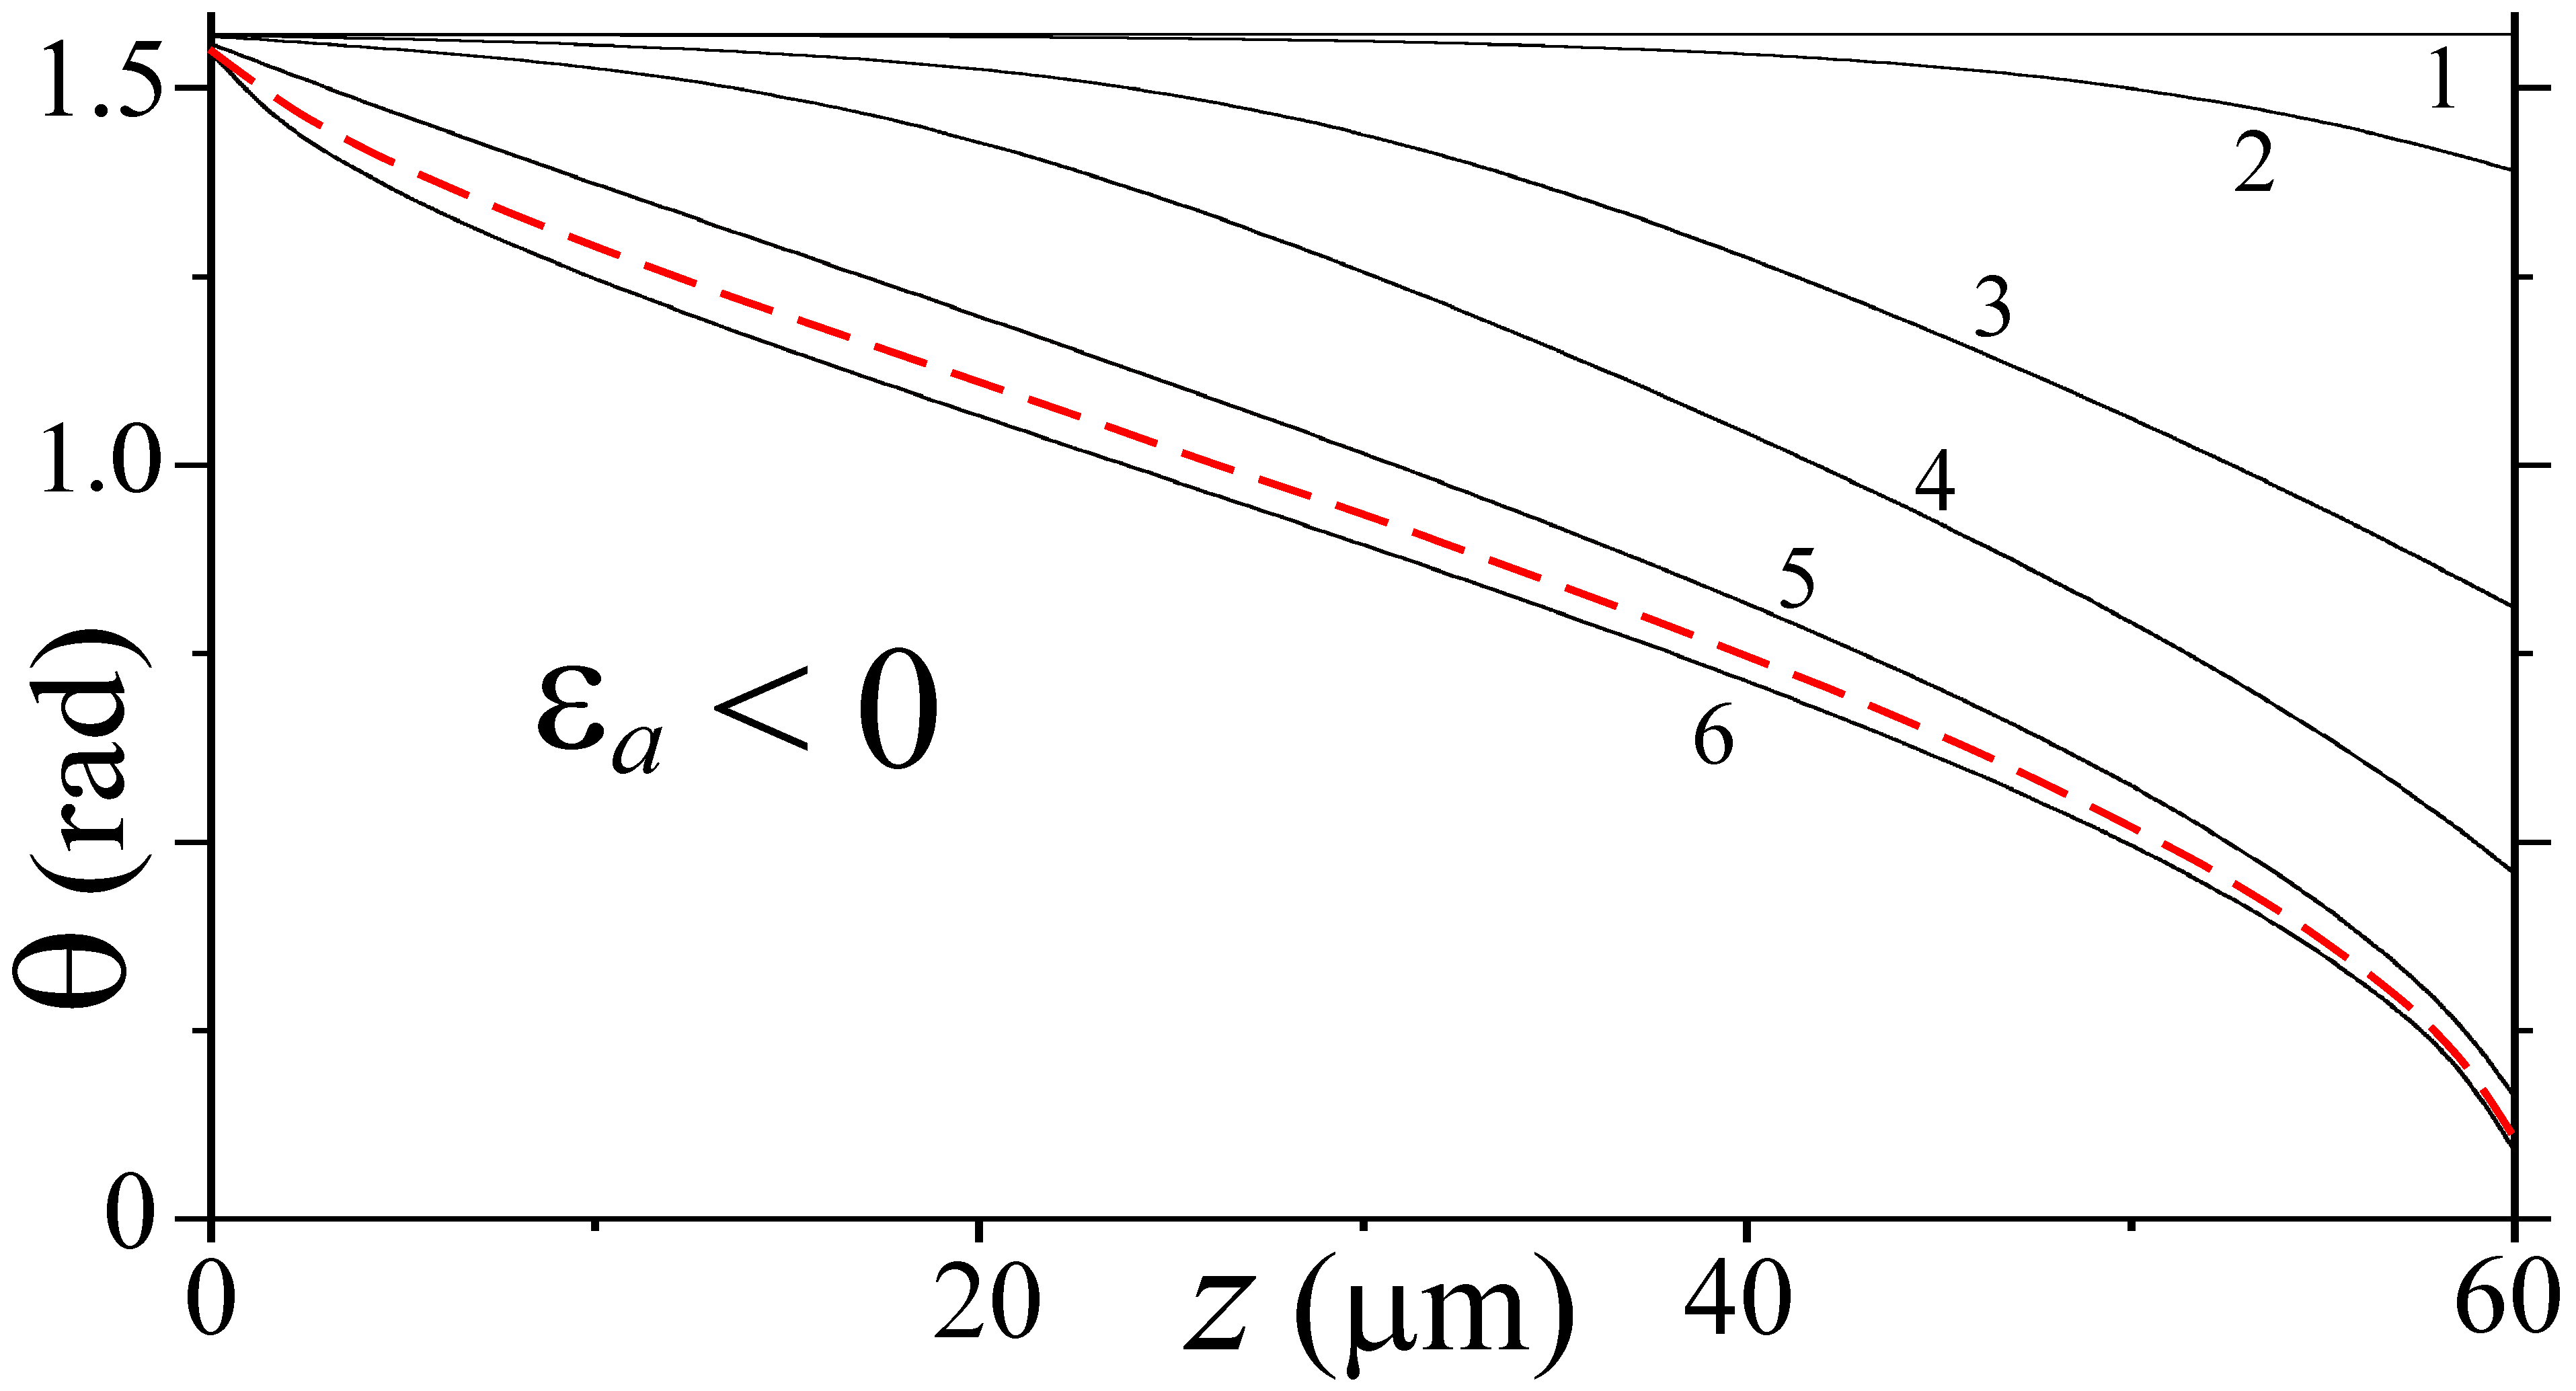
\includegraphics[width=0.49\textwidth]{Fig4_parody1a.eps}
	\hfill
	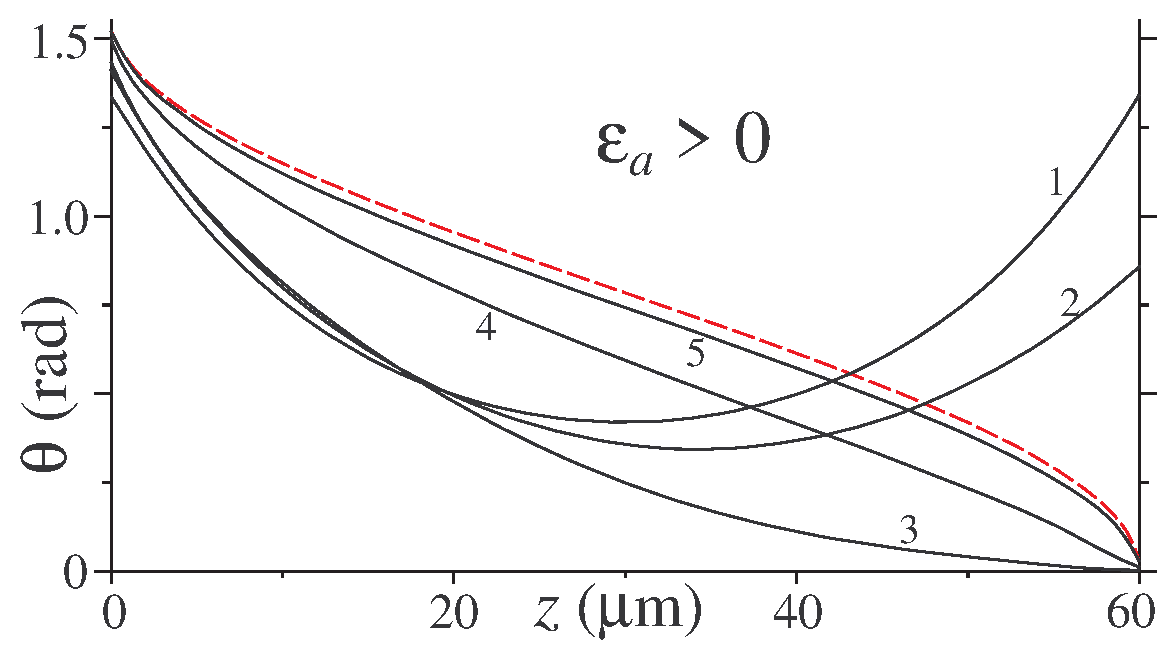
\includegraphics[width=0.49\textwidth]{symm_all_6curvesNoReflect1b.eps}
	\caption{Графики зависимости $\theta(z)$ при $U=1.2$~В.
		Значения $\bar{e}$ в единицах $\mathrm{statC/cm}$ для случая $\varepsilon_a < 0$: 1 -- $\bar{e}=10^{-3}$, 2 -- $\bar{e}=1.5\times 10^{-3}$, 3 -- $\bar{e}=1.8\times 10^{-3}$, 4 -- $\bar{e}=2\times 10^{-3}$, 5 -- $\bar{e}=3\times 10^{-3}$, 6 -- $\bar{e}=10^{-2}$; значения $\bar{e}$ при $\varepsilon_a > 0$: 1 -- $\bar{e}=0$, 2 -- $\bar{e}=10^{-4}$, 3 -- $\bar{e}=10^{-3}$, 4 -- $\bar{e}=3\times 10^{-3}$, 5 -- $\bar{e}=10^{-2}$ в единицах $\text{Фр}/\text{см}$.
		Красные пунктирные линии соответствуют зависимости $\cos^2\theta(z)\simeq {z/L}$.}\label{fig2}
\end{figure}
В случае, когда $\bar{e}$ достаточно мал, равновесные ориентационные структуры значительно отличаются для $\varepsilon_a > 0$ и $\varepsilon_a < 0$.
Однако с ростом $\bar{e}$ ориентационные структуры становятся очень схожи.
Это интересное свойство может быть объяснено следующим образом.
Выражение для свободной энергии~\eqref{eq:free-energy} при больших значениях $\bar{e}$ и/или $U$ (когда вкладами, содержащими $K_{ii}$ и $W^{(\alpha)}_{\theta,\varphi}$, можно пренебречь), сводится к следующему:
\begin{equation}\label{eq_F_f_final123}
\FF\simeq-\frac{S_{\!\bot}}{8\pi}U^2 J +S_{\!\bot} \bar{e}U JJ_1 + 2\pi S_{\!\bot} \bar{e}^2\int_{0}^{L}\frac{(\sin 2\theta \,\theta'-JJ_1)^2}{{\EE}(\theta)}dz.
\end{equation}
Рассмотрим ситуацию, когда вклады, содержащие $\bar{e}$, значительно превосходят первый вклад в~\eqref{eq_F_f_final123}.
Чтобы выяснить критерий наступления этого случая, оценим по модулю отношение второго слагаемого в~\eqref{eq_F_f_final123} к первому:
\begin{equation}\label{ch4:eq_e/U>>1}
\frac{8\pi\bar{e}UJJ_1}{U^2 J}\sim \frac{\bar{e}}{\ve_a U} \gg 1
\end{equation}
Последнее неравенство и является критерием.
Кроме того, в ситуации, когда $\sin 2\theta \,\theta'-JJ_1\neq 0$, это же неравенство означает превосходство последнего слагаемого в~\eqref{eq_F_f_final123} над остальными.
Определим, какой профиль $\theta(z)$ даёт доставляет минимум функционалу~\eqref{eq_F_f_final123}, когда выполнено условие~\eqref{ch4:eq_e/U>>1}.
Можно заметить, что интеграл в слагаемом, содержащем $\bar{e}^2$, неотрицателен, а значит, на равновесной ориентационной конфигурации $\theta(z)$ должен быть близок к нулю.
Это достигается, когда выполнено следующее равенство:
\begin{equation}
\sin 2\theta \,\theta'-JJ_1 = 0.
\end{equation}
Общим решением этого дифференциального уравнения является функция $\theta(z)$, для которой
\begin{equation}\label{ch4:eq_cos2=az+b}
\cos^2\theta(z) = az+b
\end{equation}
с произвольными константами $a$ и $b$.
Так как третье слагаемое в~\eqref{eq_F_f_final123} близко к нулю, минимум свободной энергии определяется вторым слагаемым.
Подставляя~\eqref{ch4:eq_cos2=az+b} в~\eqref{eq_F_f_final123} и опуская первое слагаемое, получаем
\begin{equation}
\FF \simeq -S_\bot \bar{e} U a.
\end{equation}
Таким образом, минимуму $\FF$ соответствует максимальное положительное значение $a$.
Для его определения учтём ограничения на $a$ и $b$, следующие из определения~\eqref{ch4:eq_cos2=az+b}:
\begin{equation}\label{ch4:eq_rectangle01}
0 \leq az + b \leq 1
\qquad \forall z\in [0,\ L]
\end{equation}
Таким образом, отрезок прямой $az+b$ на $z\in[0,\ L]$ должен целиком находиться в области, изображённой на Рис.~\ref{ch4:pic_rectangle01}, то есть его левый конец должен лежать на левой границе приведённой области, а правый -- на правой.
\begin{figure}\label{ch4:pic_rectangle01}
	\centering
	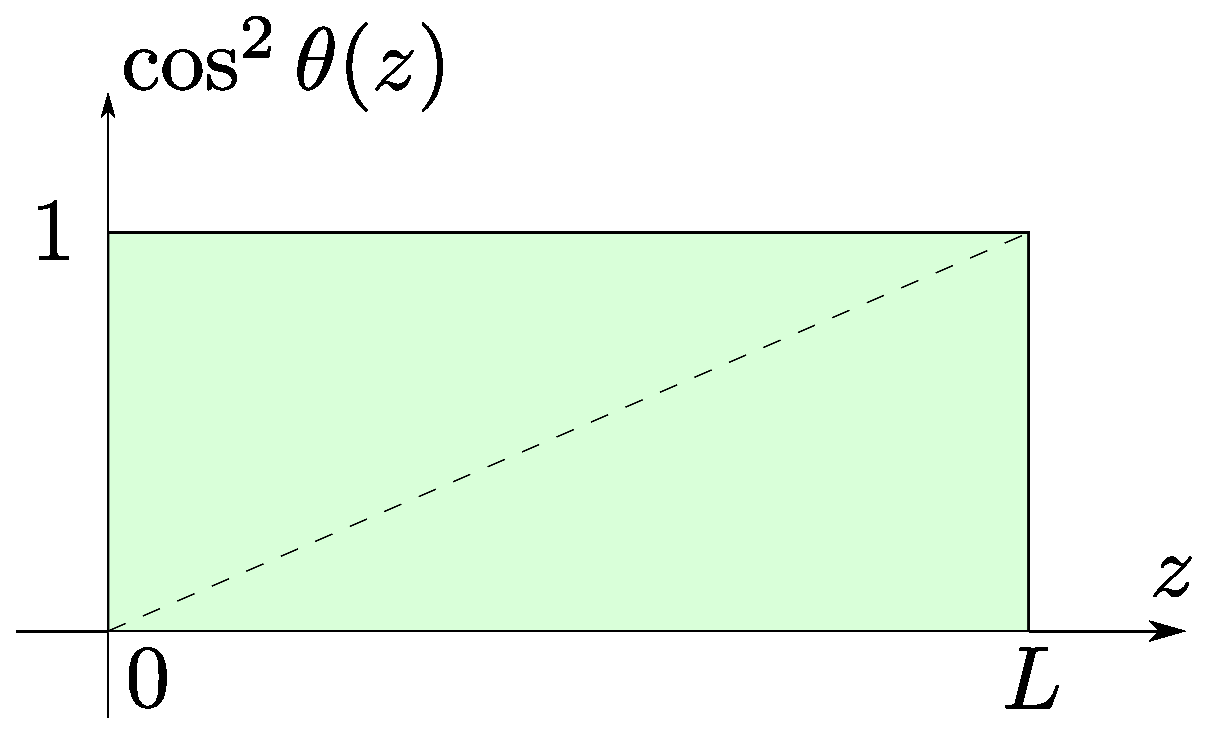
\includegraphics[width=8cm]{rectangle01}
	\caption{Область, задаваемая неравенствами~\eqref{ch4:eq_rectangle01} и отрезок прямой с наибольшим возможным угловым коэффициентом.}
\end{figure}
Нетрудно заметить, что наибольшее положительно значение $a$ соответствует прямой, отмеченной на Рис.~\ref{ch4:pic_rectangle01}  пунктиром, и равняется $1/L$, $b = 0$.
Таким образом, минимум функционала $\FF$ как при $\varepsilon_a<0$, так и при $\varepsilon_a>0$ даётся зависимостью $\cos^2\theta(z)\simeq {z/L}$.
Отметим, что при достаточно больших $\bar{e}$ равновесной является гибридно-ориентированная структура.
В такой структуре рядом с одной из границ молекулы в среднем выстраиваются параллельно ограничивающей плоскости, а рядом с другой -- перпендикулярно. ~\todo{можно вставить красивый рисунок-иллюстрацию.}
Такой переход между планарной геликоидальной и гибридной структурами может быть использован для создания переключателей, в основе работы которых лежит флексоэлектричество.

Кроме того, в ячейке ХЖК с достаточно большим $\bar{e}$ был обнаружен ориентационный переход нового типа.
Такой переход продемонстрирован на Рис.~\ref{fig4_3}, где представлены профили $\theta(z)$ при фиксированном $\bar{e}$ и различных значениях напряжения $U$.
С ростом приложенного напряжения от нулевого значения сначала происходит непрерывный переход Фредерикса.
При дальнейшем увеличении напряжения происходит ещё один переход.
Этот переход является разрывным, так как происходит между двумя значительно различающимися ориентационными структурами.
Это иллюстрируют графики 2 и 3 на Рис.~\ref{fig4_3}: разница в приложенном напряжении составляет $0.01$~В, при этом полученные профили существенно различны.
\begin{figure}
	\centering
	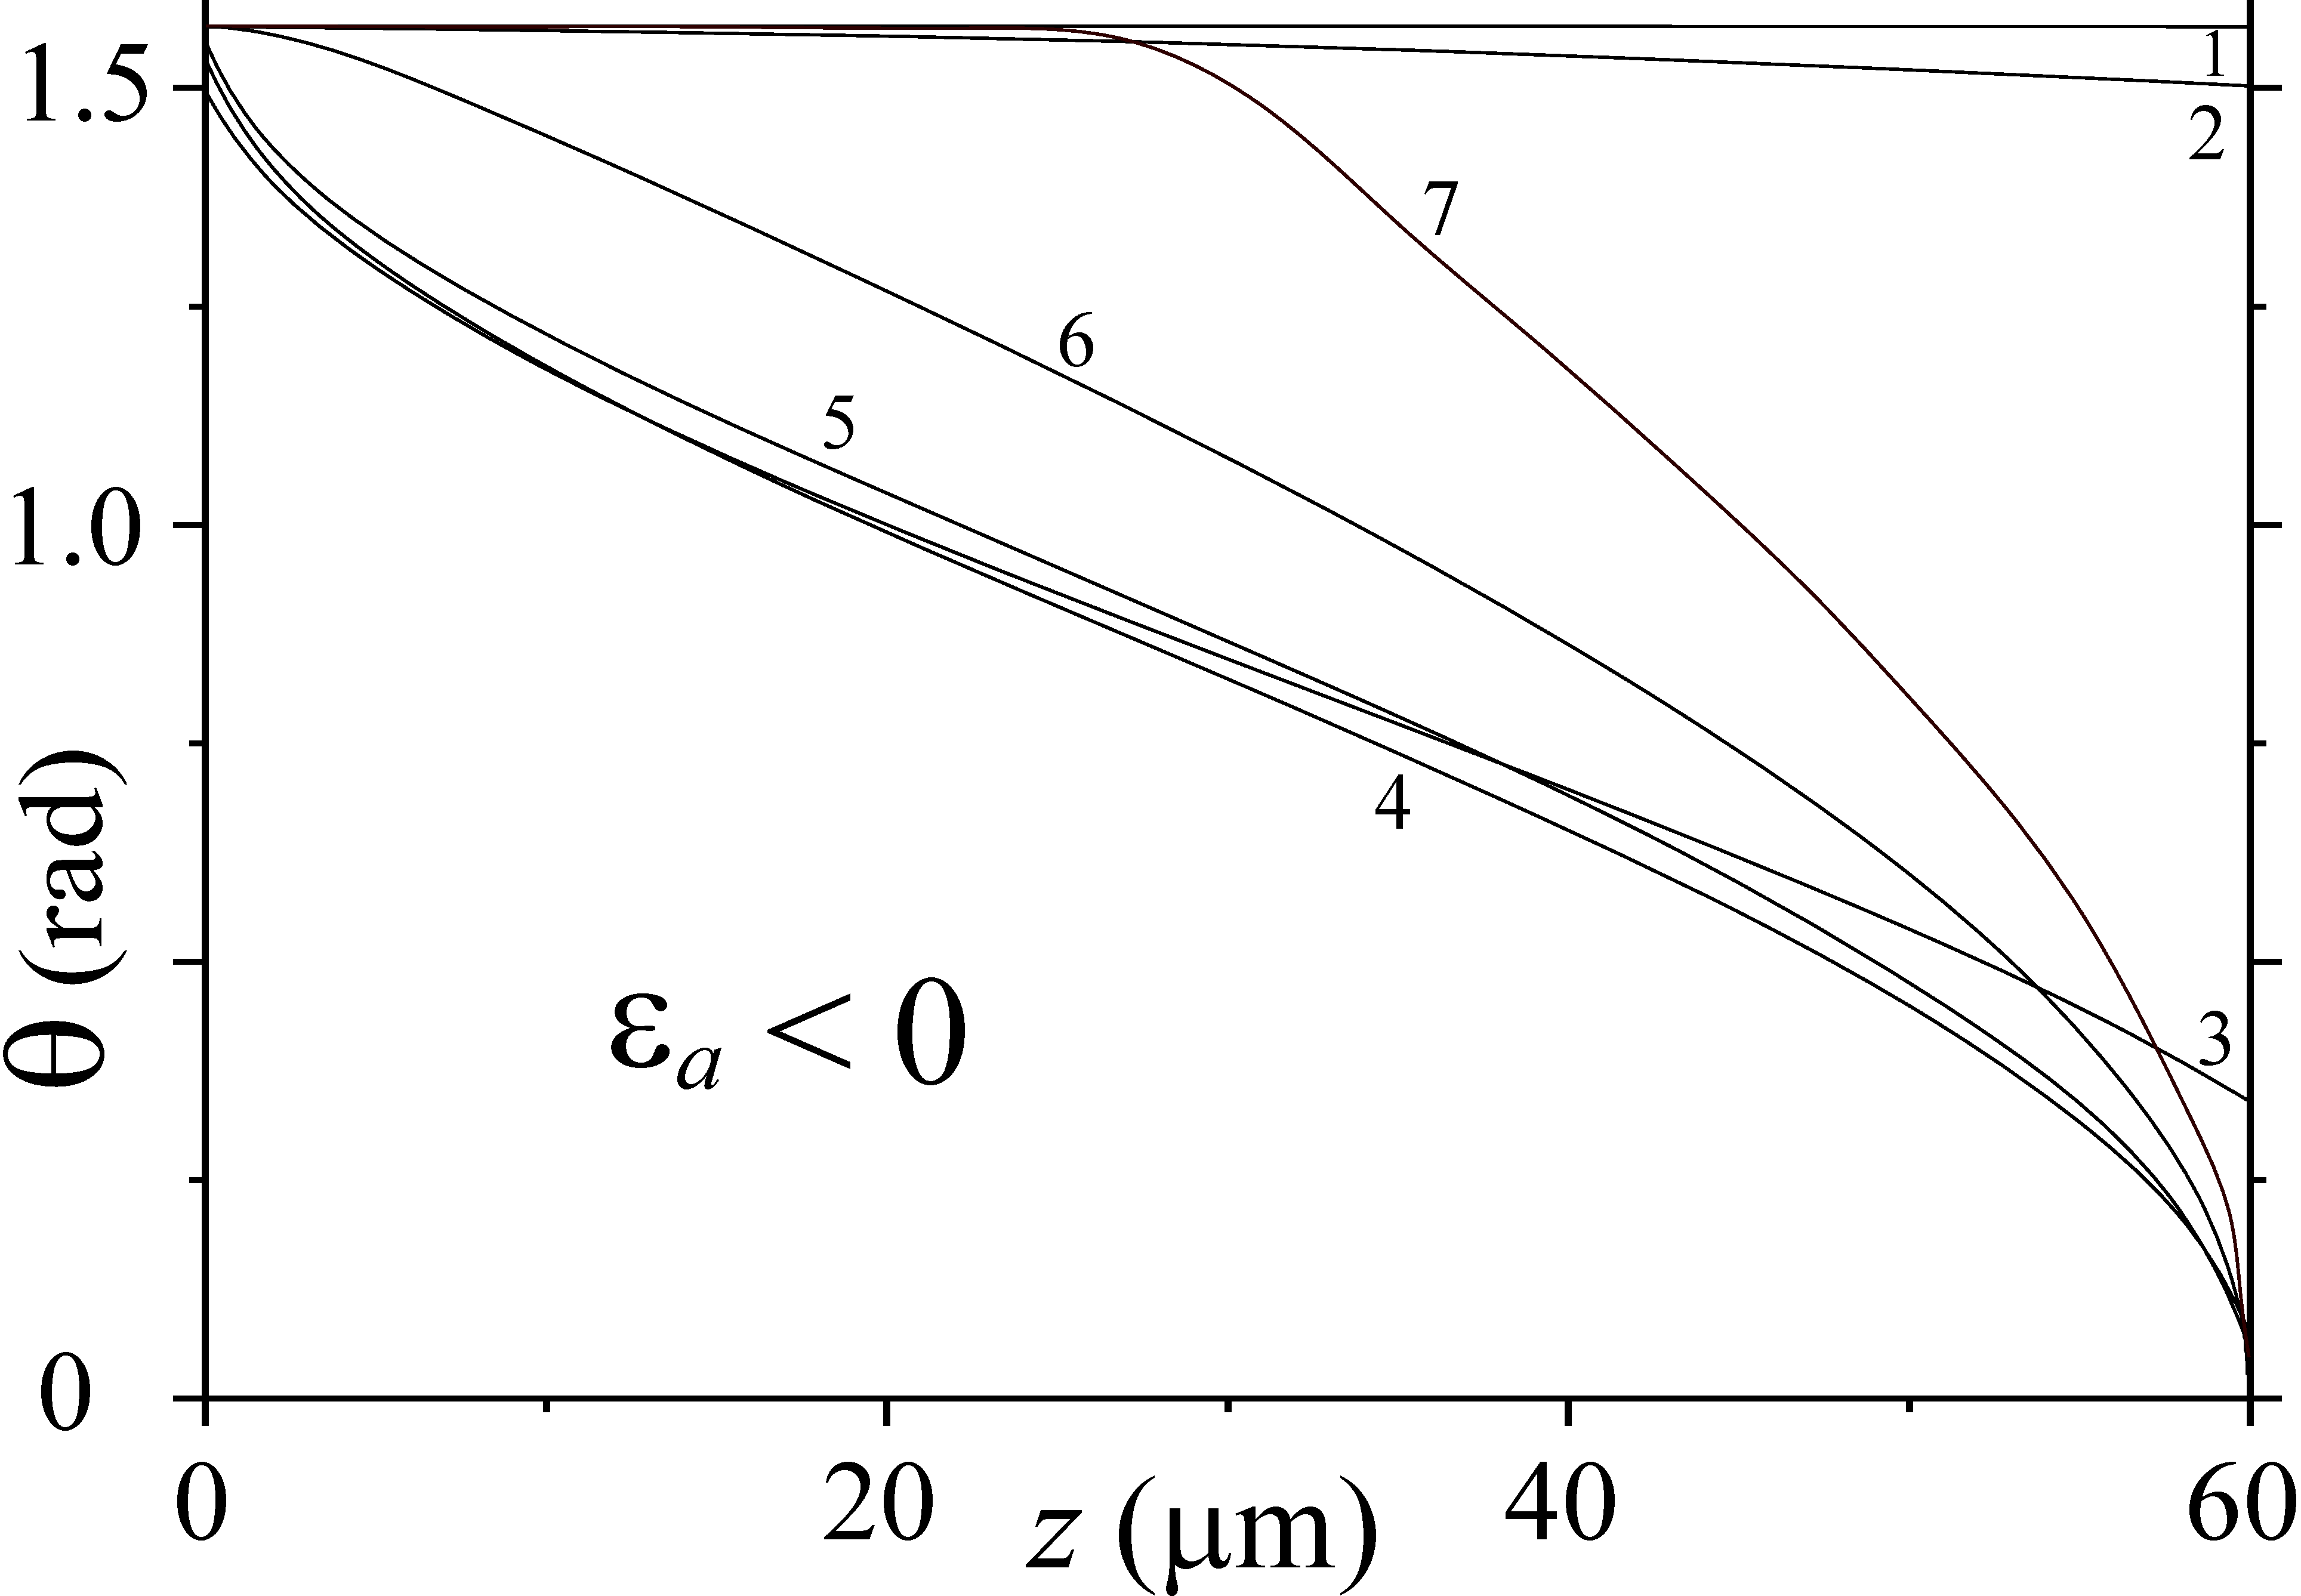
\includegraphics[width=0.48\textwidth]{Profiles_at_fixed_e_0_01_change_U.eps}%\\
	\hfill
	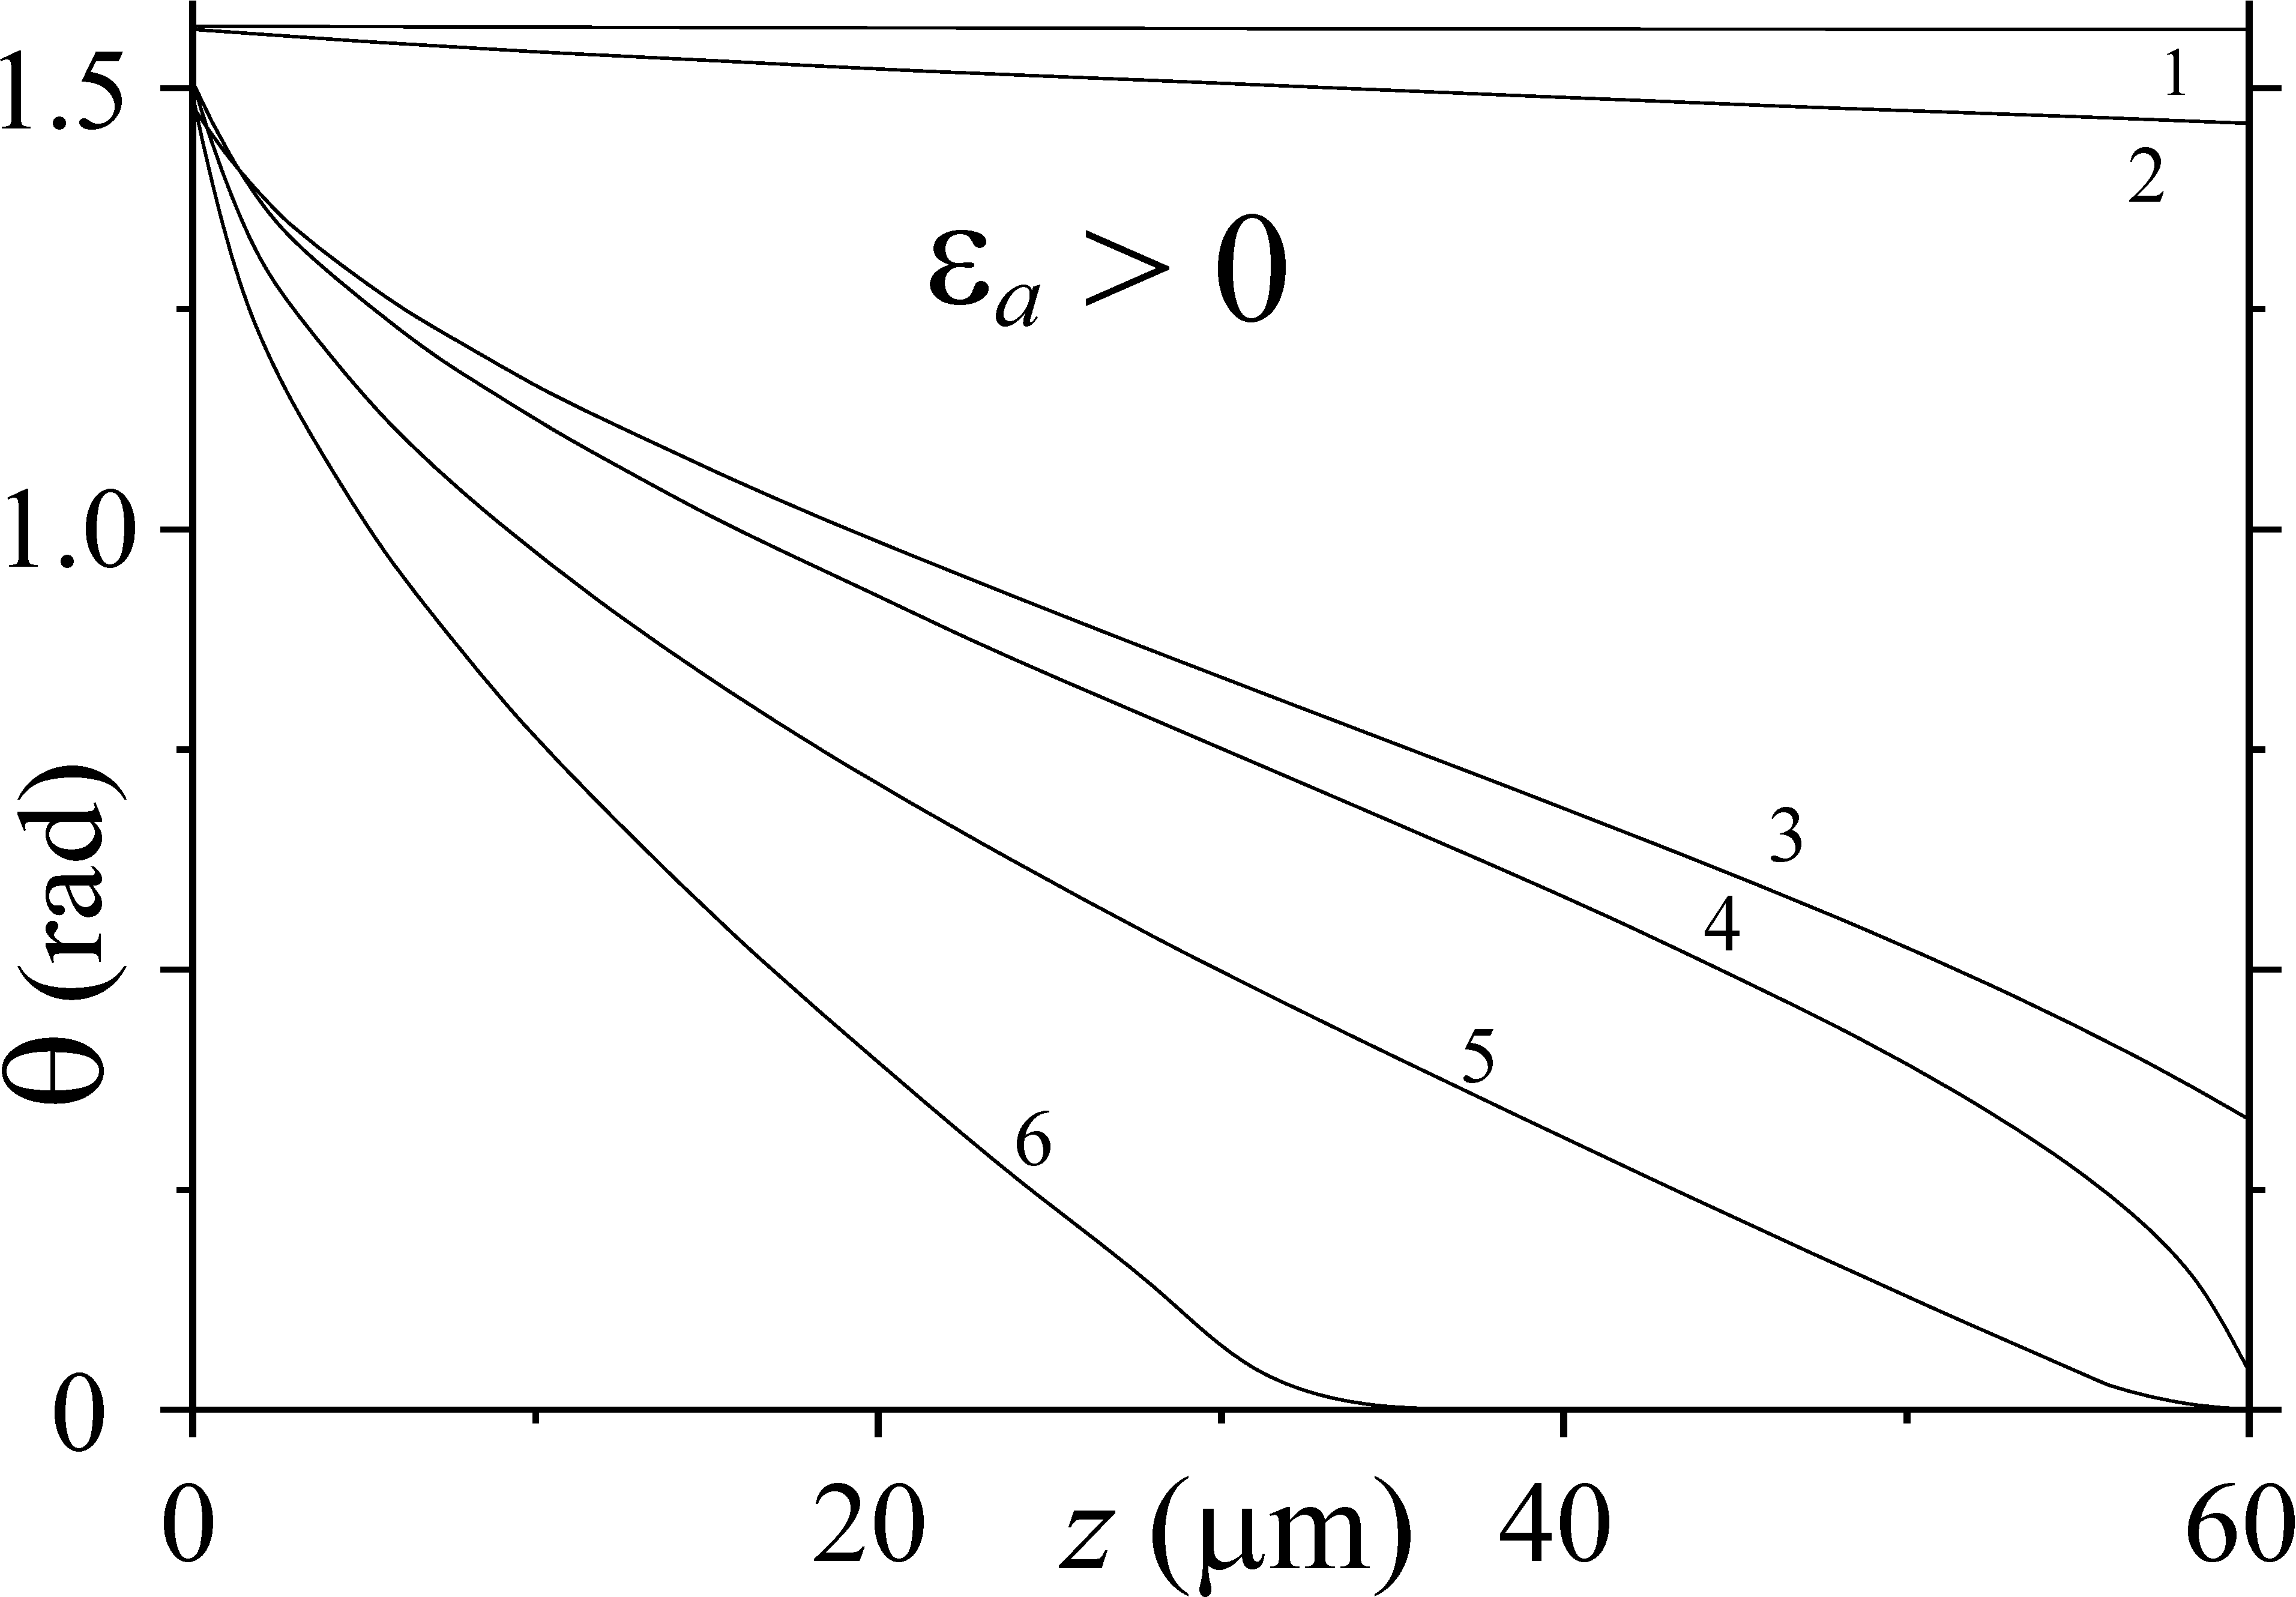
\includegraphics[width=0.48\textwidth]{Profiles_POSITIVE_EA_at_fixed_e_0_01_change_U.eps}
	\caption{Равновесная ориентационная структура $\theta(z)$ при $\bar{e}=0.01$~Фр/см. Напряжения для случая $\varepsilon_a<0$: 1 -- $U=0.15$~В, 2 -- $U = 0.17$~В, 3 -- $U = 0.18$~В, 4 -- $U = 1$~В, 5 -- $U = 2$~В, 6 -- $U = 5$~В и 7 -- $U = 10$~В; для случая $\varepsilon_a > 0$: 1 -- $U = 0.15$~В, 2 -- $U = 0.17$~В, 3 -- $U = 0.18$~В, 4 -- $U = 1$~В, 5 -- $U = 5$~В и 6 -- $10$~В.}\label{fig4_3}
\end{figure}
Отметим, что при очень высоком напряжении $U$ первое слагаемое в выражении~\eqref{eq_F_f_final123} становится определяющим.
Следовательно, система стремится к насыщенной ориентационной структуре, которая описывается зависимостью $\theta(z) = \pi/2$ при $\varepsilon_a < 0$ и $\theta(z) = 0$ при $\varepsilon_a > 0$.
Это можно пронаблюдать на Рис.~\ref{fig4_3} на примере профилей 5-7 для случая $\ve_a < 0$ и профилей 5 и 6 для случая $\ve_a > 0$.